% Created 2018-10-08 Mon 04:35
% Intended LaTeX compiler: pdflatex
\documentclass[presentation,12pt]{beamer}
\usepackage[utf8]{inputenc}
\usepackage[T1]{fontenc}
\usepackage{graphicx}
\usepackage{grffile}
\usepackage{longtable}
\usepackage{wrapfig}
\usepackage{rotating}
\usepackage[normalem]{ulem}
\usepackage{amsmath}
\usepackage{textcomp}
\usepackage{amssymb}
\usepackage{capt-of}
\usepackage{hyperref}
\usetheme{Hannover}
\author{Matheus Artur, Luís Alberto Cabús, Nicolas Leão, Fábio Vinícius}
\date{\url{https://github.com/projetosufal/data-structures-project}}
\title{Segment Tree}
\hypersetup{
 pdfauthor={Matheus Artur, Luís Alberto Cabús, Nicolas Leão, Fábio Vinícius},
 pdftitle={Segment Tree},
 pdfkeywords={},
 pdfsubject={},
 pdfcreator={Emacs 26.1 (Org mode 9.1.9)}, 
 pdflang={English}}
\begin{document}

\maketitle
\begin{frame}{Outline}
\tableofcontents
\end{frame}


\section{Introduction}
\label{sec:org5f3c0ad}

\begin{frame}[label={sec:orgcd2b5b6}]{Stock Exchange}
\begin{columns}
\begin{column}{0.48\columnwidth}
\begin{block}{The problem}
\begin{itemize}
\item Data from thousands of companies worldwide, active for decades
\item Usage of multiple operations requiring da range/interval of time required
\item Efficiency demand
\end{itemize}
\end{block}
\end{column}

\begin{column}{0.48\columnwidth}
\begin{block}{O(n) operations?}
\begin{center}
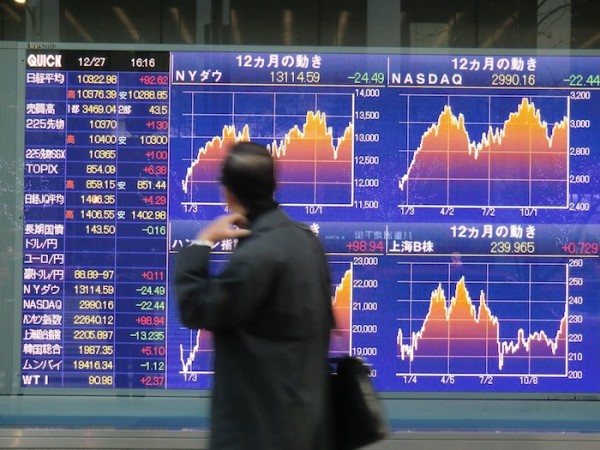
\includegraphics[width=.9\linewidth]{./img/serv.png}
\end{center}
\end{block}
\end{column}
\end{columns}
\end{frame}
\section{Segment tree}
\label{sec:org4060469}
\begin{frame}[label={sec:org2b8c3d6}]{Segment tree}
\begin{block}{How it is structured?}
The Segtree is a binary tree that's represented from a array, where each node represents a unique interval or segment of the tree and stores a \alert{specific} value. 
\end{block}
\begin{block}{For what purpose?}
The value, are usually represented by \emph{maximum}, \emph{minimum} or \emph{sum} of the segment. The goal is acess these values as a search within a range.
\end{block}
\end{frame}
\begin{frame}[label={sec:org9dacd48}]{}
\begin{center}
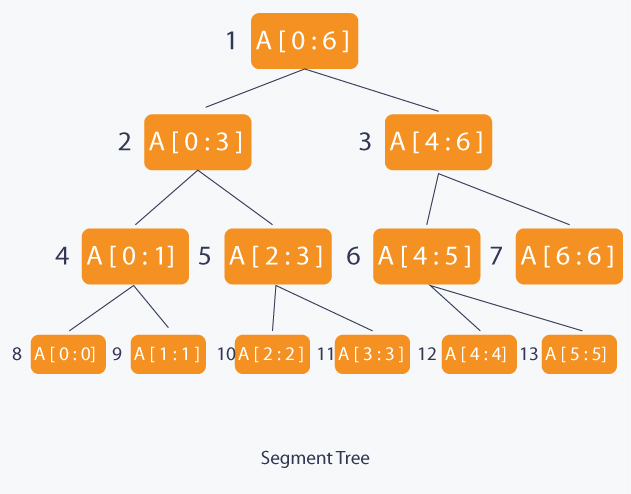
\includegraphics[width=.9\linewidth]{./img/segtree.jpg}
\end{center}
\end{frame}
\begin{frame}[label={sec:org7f7c3f7}]{}
\end{frame}
\end{document}
